\newpage
\section{EMC}
Tijdens de lessen van het vak zijn manier behandelt om ervoor te zorgen dat systemen minder beïnvloed worden door elektromagnetische signalen van buiten af. Tijdens het ontwerpen van deze applicatie is er geprobeerd rekening te houden met deze informatie. Dit is gedaan door alle connector van de sensor PCB aan één kant te plaatsen. Hierdoor wordt de PCB niet een dipole antenne en pikt hij minder Elektromagnetische straling op. Een weergave van de PCB is weergegeven in Figuur \ref{fig:PCB_render}.
\begin{figure}[H]
    \centering
    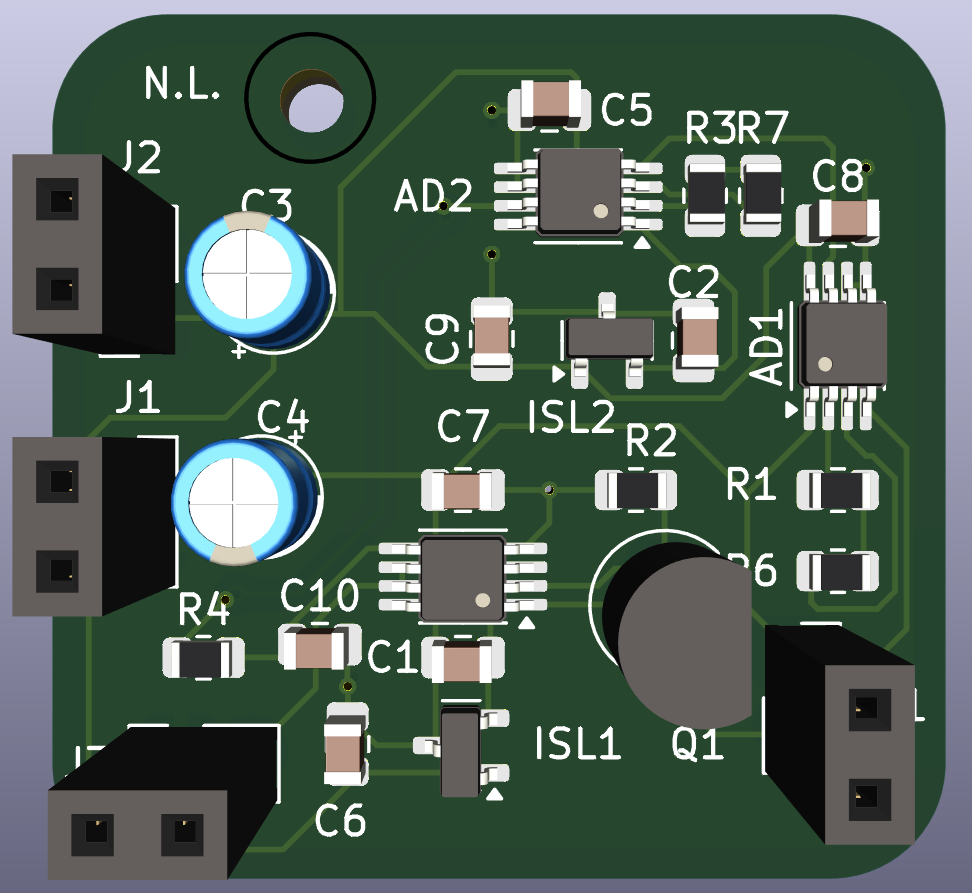
\includegraphics[width=0.75\linewidth]{pictures/pcb_render.png}
    \caption{De ontworpen PCB voor de temperatuur sensor die direct op de ADC en voedingen aangesloten kan worden.}
    \label{fig:PCB_render}
\end{figure}